\documentclass[10pt, a4paper, english]{../Template/NTNUoving}
\usepackage[utf8]{inputenc}
\usepackage[T1]{fontenc}
\usepackage{float}
\usepackage{enumitem}
\usepackage{csquotes}
\usepackage{algorithm}
\usepackage{algorithmic}
\usepackage{listings}
\usepackage{listings}
\usepackage{color}
\usepackage{biblatex}
\usepackage{hyperref}
\ovingnr{1}    % Nummer på innlevering
\semester{Spring 2021}
\fag{Methods in Artificial Intelligence \\ TDT4171}
\institutt{Department for Computer Science}

\begin{document}

% Problem 1
\begin{oppgave}

    % a
    \begin{punkt}
        \begin{align*}
            P(Siblings \leq 2)
            &= P(Siblings = 0) + P(Siblings = 1) + P(Siblings = 2) \\
            &= 0.15 + 0.49 + 0.27 \\
            &= 0.91
        \end{align*}
    \end{punkt}

    % b
    \begin{punkt}
        \begin{align*}
            P(Siblings > 2 | Siblings \geq 1)
            &= \frac{P(Siblings > 2 \wedge Siblings \geq 1)}{P(Siblings \geq 1)} \\
            &= \frac{P(Siblings > 2)}{P(Siblings \geq 1)} \\
            &= \frac{1-P(Siblings \leq 2)}{1-P(Siblings = 0)} \\
            &= \frac{0.09}{0.85} = \frac{9}{85} \approx 0.1059
        \end{align*}
    \end{punkt}

    % c
    \begin{punkt}
        Let $S_1$, $S_2$ and $S_3$ denote the siblings for each of the friends.

        There are 3 permutations for who can have 3 siblings and the other 0 siblings,
        only 1 permutation where each have 1 sibling and $3\cdot2=6$ permutations for who can have 2 siblings, 1 sibling and 0 sibling
        (we first have 3 choices for the friend with 2 siblings, then 2 choices for the one with 1 sibling).
        This gives us:

        \begin{align*}
            P(S_1 + S_2 + S_3 = 3)
            &= 3P(S_1 = 3)P(S_2 = 0)P(S_3 = 0) \\
            &+ P(S_1 = 1)P(S_2 = 1)P(S_3 = 1) \\
            &+ 6P(S_1 = 2)P(S_2 = 1)P(S_3 = 0) \\
            &= 3\cdot0.06\cdot0.15^2 + 0.49^3 + 6\cdot0.27\cdot0.49\cdot0.15\\
            &= 0.240769
        \end{align*}
    \end{punkt}

    % d
    \begin{punkt}
        Let $S_E$ and $S_J$ denote siblings for Emma and Jacob respectfully. We have:
        \begin{align*}
            P(S_E = 0 | S_E + S_J = 3)
            &= \frac{P(S_E = 0 \wedge S_E + S_J = 3)}{P(S_E + S_J = 3)} \\
            P(S_E = 0 \wedge S_E + S_J = 3) &= P(S_E = 0)P(S_J = 3) \\
            P(S_E + S_J = 3) &= 2 P(S_E = 0)P(S_J = 3) + 2 P(S_E = 1)P(S_J = 2) \\
            \implies P(S_E = 0 | S_E + S_J = 3) &= \frac{P(S_E = 0)P(S_J = 3)}{2 P(S_E = 0)P(S_J = 3) + 2 P(S_E = 1)P(S_J = 2)} \\
            &= \frac{0.15\cdot0.06}{2\cdot0.15\cdot0.06 + 2\cdot0.49\cdot0.27} \\
            &= \frac{5}{157} \approx 0.031847
        \end{align*}
    \end{punkt}
\end{oppgave}

% Problem 2
\begin{oppgave}
    %a
    \begin{punkt}
        Every node can be represented by $2^k$ numbers where $k$ is the number of parent nodes when each variable has a Boolean state.
        This gives us the following:
        \begin{center}
            \begin{tabular}{ |c|c| }
             \hline
             Variable & Numbers needed \\
             \hline
             A  & 1 \\
             \hline
             B &  2 \\
             \hline
             C &  2 \\
             \hline
             D &  2 \\
             \hline
             E &  4 \\
             \hline
             F &  4 \\
             \hline
             G &  2 \\
             \hline
             H &  1 \\
             \hline
             Sum &  18 \\
             \hline
            \end{tabular}
            \end{center}
            As we can see the sum is 18 numbers needed and the statement is thus \textbf{true}.
    \end{punkt}

    % A node X is conditionally independent of its non-descendants given its parents.
    % A node X is conditionally independent of all othr nodes in the network given its Market blanket.
    % Markov blanket: Parents, children and children's parents
    % b
    \begin{punkt}
        \textbf{False}, since both $G$ and $A$ have $E$ as an descendant and we are not given any evidence they are not independent.
    \end{punkt}

    % c
    \begin{punkt}
        \textbf{False}, since $E$ is not given both its parents it can't be conditionally independent from $H$.
    \end{punkt}

    % d
    \begin{punkt}
        \textbf{True}, since $E$ is given both its parents it is conditionally independent from $H$.
    \end{punkt}
\end{oppgave}

% Problem 3
\begin{oppgave}

    % a
    \begin{punkt}
        \begin{align*}
            P(b) &=
            P(b|a)P(a)+P(b|\neg a)P(\neg a) \\
            &= 0.44 \\
            \implies P(\neg b) &= 1-P(b) = 0.56
        \end{align*}
    \end{punkt}

     % b
     \begin{punkt}
        \begin{align*}
            P(d) &=
            P(d|b)P(b)+P(d|\neg b)P(\neg b) \\
            &= 0.712 \\
        \end{align*}
     \end{punkt}

      % c
    \begin{punkt}
        \begin{align*}
            P(B | \neg d)
            &= \alpha \langle P(\neg d|b)P(b), P(\neg d | \neg b)P(\neg b) \rangle \\
            &= \alpha \langle \frac{22}{125}, \frac{14}{125} \rangle = \langle \frac{11}{18}, \frac{7}{18}\rangle \\
            \implies P(c|\neg d) &= P(c|b)P(b|\neg d) +  P(c|\neg b)P(\neg b|\neg d) \\
            &= \frac{11}{180} + \frac{7}{60} = \frac{8}{45} \approx 0.178
        \end{align*}
        $\alpha$ is the normalizing factor.
    \end{punkt}

     % d
     \begin{punkt}
        \begin{align*}
            P(A | \neg c, d)
            &= \alpha \langle P(a)\sum_b P(\neg b|a)P(\neg c |b) P(d|b), P(\neg a)\sum_b P(\neg b|\neg a)P(\neg c |b) P(d|b) \rangle \\
            &= \alpha \langle \frac{11}{25}, \frac{139}{1250} \rangle = \langle \frac{550}{689}, \frac{139}{689} \rangle \approx \langle 0.7983, 0.2017 \rangle
        \end{align*}
        $\alpha$ is the normalizing factor.
     \end{punkt}
\end{oppgave}
\clearpage
% Problem 4
\begin{oppgave}
    % c
    \setcounter{Punkt}{2}
    \begin{punkt}
        The Monty-Hall problem can be described by a bayesian network where $OpenedByHost$ is conditional based on $Prize$ and $ChosenByGuest$:

        \begin{figure}[h]
            \centering
            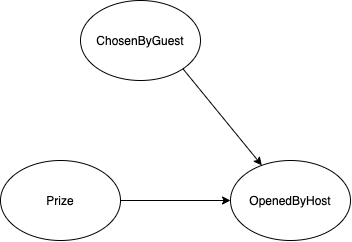
\includegraphics[width=0.5\textwidth]{BN.png}
            \caption{Bayesian network for the Monty Hall-problem.}

            \end{figure}

        The conditional probability tables are given by:
        \begin{table}[h!]
            \centering
            \begin{tabular}{|c|c|}
                \hline
                & $P(Prize)$ \\ [0.5ex]
                \hline
                $Door1$ & 0.333 \\ [1.0ex]
                $Door2$ & 0.333 \\ [1.0ex]
                $Door3$ & 0.333 \\ [1.0ex]
                \hline
            \end{tabular}
            \caption{Probability distribution for $Prize$.}
        \end{table}

        \begin{table}[h!]
            \centering
            \begin{tabular}{|c|c|}
                \hline
                & $P(ChosenByGuest)$ \\ [0.5ex]
                \hline
                $Door1$ & 0.333 \\ [1.0ex]
                $Door2$ & 0.333 \\ [1.0ex]
                $Door3$ & 0.333 \\ [1.0ex]
                \hline
            \end{tabular}
            \caption{Probability distribution for $ChosenByGuest$.}
        \end{table}

        \begin{table}[h!]
            \centering
            \begin{tabular}{|c|c|c|c|c|c|c|c|c|c|}
                \hline
                $Prize$ & 0 & 1 & 2 & 0 & 1 & 2 & 0 & 1 & 2 \\ [1.0ex]
                $ChosenByGuest$ & 0 & 0 & 0 & 1 & 1 & 1 & 2& 2 & 2 \\ [1.0ex]
                \hline
                $Door1$ & 0 & 0 & 0 & 0.5 & 0.5 & 1 & 0 & 1  & 0.5 \\ [1.0ex]
                $Door2$ & 0.5 & 0 & 1 & 0 & 0 & 0 & 1 & 0 & 0.5 \\ [1.0ex]
                $Door3$ & 0.5 & 1 & 0 & 0.5 & 0.5 & 0 & 0 & 0 & 0 \\ [1.0ex]
                \hline
            \end{tabular}
            \caption{Probability distribution for $ChosenByGuest$.}
        \end{table}

        \begin{align*}
            P(Prize | ChosenByGuest = 1, OpenedByHost = 3) &= \langle 0.3333, 0.6667, 0.0000 \rangle
        \end{align*}
        Based on this it is of the interest of the guest to switch their choice.
    \end{punkt}
\end{oppgave}
\end{document}